%!TEX root = ../template.tex
%%%%%%%%%%%%%%%%%%%%%%%%%%%%%%%%%%%%%%%%%%%%%%%%%%%%%%%%%%%%%%%%%%%%
%% chapter3.tex
%% NOVA thesis document file
%%
%% Chapter with a short laext tutorial and examples
%%%%%%%%%%%%%%%%%%%%%%%%%%%%%%%%%%%%%%%%%%%%%%%%%%%%%%%%%%%%%%%%%%%%
\chapter{Approach of Elaboration Phase}
\label{cha:approach_of_elaboration_phase}

In this chapter we present an initial overview of the system model, as well as some inicial guidelines planned to be implemented to our solution during the elaboration phase, while reinforcing the main objectives of this thesis.

\section{Addressing the objectives and contributions} % (fold)
\label{sec:document_structure}

The solution we are going to implement and study in this thesis has the purpose of allowing unmodified applications to run in trustable commodity hardware without any major performance overheads, comparing it to applications running without this extra sense of security. To implement this, we are focusing on three fulcral points:
\begin{itemize}
	\item \textbf{Descentralization:}  Adding redundancy to the storage and processing of data, increasing the system availability and reliability;
	\item \textbf{Reduction of TCB size:}  Making each node of the system only trust what is essencial to its normal execution, leaving the rest out of the \gls{tcb} will increase the overall security of the system;
	\item \textbf{Data privacy:}  Assuring that data remains private while stored and processed, by finding a way to keep the data encrypted, protecting it from entities that are not supposed to access it.
\end{itemize}
By achieving this, we hope to deliver a full-fledged solution, capable of granting privacy and security to data inside dependable systems.




\section{System Model Overview} % (fold)
\label{sec:dealing_with_bibliogrpahy}

Our system model is composed in three main components: a client, a processing layer made of a \gls{kvs} that will be responsible of storing and processing data at runtime, and a storage layer. For a better grasp of the system as a whole, we can analyse the Figure \ref{fig:systemModel}.

\begin{figure}[htbp]
	\centering
	{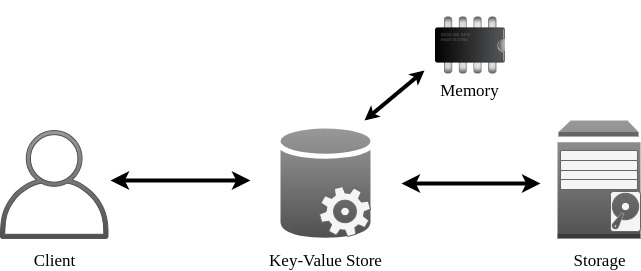
\includegraphics[width=0.4\linewidth]{SystemModelFinal}}
	\caption{Overview of the System Model}
	\label{fig:systemModel}
\end{figure}

The client layer is going to consist of a benchmark application responsable of making requests to the \gls{kvs}, while evaluating certain defined metrics that will be used on our experimental analysis.
The processing layer, as mentioned before, will be accountable of storing and processing the data while executing, making use of volatile memory that should be protected during this phase.
As for the storage layer, we will use a \gls{raid} based persistent storage system as a way to increase redundancy, thus adding fault-tolerance and enabling faster operations over this third layer.




\section{Adversary Model} % (fold)
\label{sec:inserting_tables}

We prevent interventions made by System Administrators on Nodes from having any
effect on the computations of users. This means we want to avoid having System Admin-
istrators on a node with computations running, however we want to avoid interrupting

the computations or degrading its throughput. If interruptions or degradation happen,
we have to make sure these are as small as possible.
We assume all nodes in the infrastructure have TPMs in their hardware architectures,
and these work correctly, properly providing the functions as we described in the Chapter
2. Only the TPM possesses the proposer TPM’s private keys in validated certification
chains. Any recipient of the booted configuration (composed by the BIOS configuration,
the bootloader, Host OS and all the relevant software components in the Host OS level)
can use the TPM’s public key and the certification chain (ending in a root of trust) to
verify the related signatures.
We assume that all nodes in the infrastructure are equipped with Intel SGX enabled

CPUs and the necessary firmware support at the Host OS support level, which is con-
tained in the TCB of the solution.

PaaS software or SaaS applications should be deployed with minimal interaction (e.g.
using Preboot eXecution Environment) as stock images and, is assumed correct as far
as promised functionality and security are concerned. As we will target on Dockerized
images, we consider that Docker does not corrupt applications and is able to contain
them, with fully execution isolation. Current cryptographic protocols and standards, as


\section{Isolation and Containerization} % (fold)
\label{sec:importing_images}

Since our objectives are pointed towards an isolated system capable of offering security and privacy properties, we depend a lot on isolation techniques to make this possible, provided by hardware or software (containers). 

As for hardware isolation, we need to look at approaches capable of assuring both computation and storage security to our system's data during runtime. There are several technologies that implement \gls{tee}s that were proven to be capable of doing just that.
Also, adding to that, by using a container we will grant an extra layer of isolation to the system, as well as ease in the deployment of software running inside the container, whether it is an \gls{os}, a library \gls{os} or even entire applications.

% section importing_images (end)

\section{System Generalization} % (fold)

Looking at our system model introduced in \ref{fig:systemModel}, there are some potencial threats that need to be taken care of. 
First, the connection between the client and the \gls{kvs} need to be secured. Secondly, the data being stored at the storage layer need to be encrypted, otherwise it can be accessed and read, or even stolen. Lastly, considering only one \gls{kvs} will induce into a single point of failure on the processing layer. Also, the data stored and running inside this layer and its memory need to be secured.

This can be achieved by using \gls{tls} over the \gls{http} protocol, securing the communication between the client and the \gls{kvs} layer.  Existing \gls{fde} technology can be used to encrypt the data to be stored in the storage layer. Finally for the processing layer, we will use a cluster of \gls{kvs}, thus adding redundancy and load balancing. As for the security and privacy concerns, by isolating each cluster replica inside individual \gls{tee}s, we achieve confidentiality and privacy of the data during runtime. The figure \ref{fig:systemModelCluster} shows an overall idea of this proposed solutions.

\begin{figure}[htbp]
	\centering
	{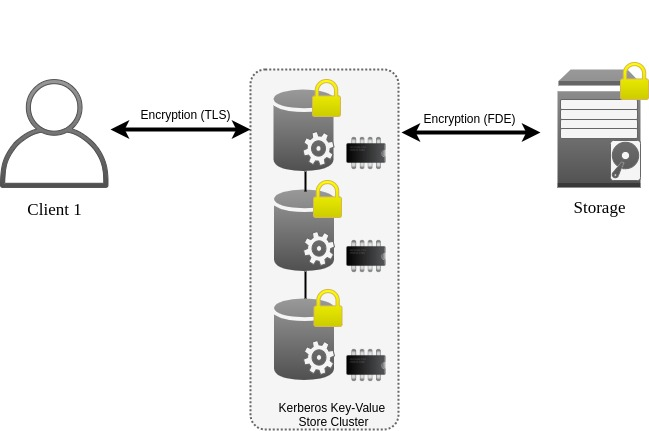
\includegraphics[width=0.4\linewidth]{SystemModelWithCluster}}
	\caption{System Model with a Key-Value Store Cluster}
	\label{fig:systemModelCluster}
\end{figure}

As a way to scale the overall system to modern requirements, we opted to divide it into two parts, one being the client layer and the other being both the processing and storage layers, which will both be implemented inside a cloud system. With this approach (figure \ref{fig:systemModelCloud}) we will guarantee scalability of the resources for the solution.

\begin{figure}[htbp]
	\centering
	{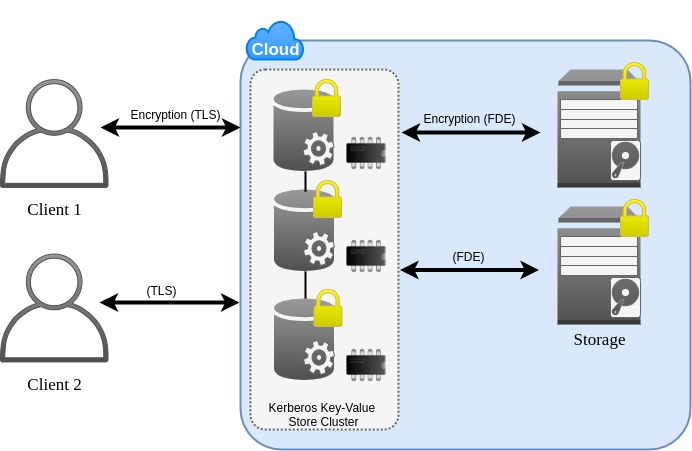
\includegraphics[width=0.4\linewidth]{SystemModelCloud}}
	\caption{System Model running inside a Cloud System}
	\label{fig:systemModelCloud}
\end{figure}

\section{Implementation Guidelines} % (fold)

For the development phase of this dissertation, and as we mentioned before in \ref{sec:objectiveAndContibutions}, we considered the following guidelines:

\textbf{Key-Value Store}: we opted for Redis due to being the most popular \gls{kvs} at the moment, as we can see in \cite{rankingKVStores}. Adding this to the fact that it fits our system needs, we thought that an exhaustive study over this technology running in a dependable system would be an interesting contribution.

\textbf{Trusted Execution Environment}: as mentioned before, we choose to go with Intel-\gls{sgx} (\ref{ssec:intelsgx}), since it offers the possibility to isolate code inside multiple enclaves, while executing on commodity hardware. Thus, we can run each node of our \gls{kvs} cluster inside of an individual enclave, assuring confidentiality and privacy of the data during runtime.

\textbf{OS library}: to run unmodified applications on top of Intel-\gls{sgx}, we picked Graphene-SGX (\ref{ssec:grapheneSGX}) as it was proven to be able to keep decent levels of performance in a system.

\textbf{Containerized OS Virtualization}: we choose Graphene-SGX Secure Container (GSC) due to being an open-source container system where an application can be protected by Intel-\gls{sgx} while running inside a container. We thought it to be a good way of adding an extra layer of isolation to the execution of each \gls{kvs} instance, while still running with the benefits of Graphene-SGX and Intel-\gls{sgx}.

\textbf{Cloud Infrastructure}: OVH \cite{ovhCloud} was the cloud provider chosen, mainly due to the fact that it supports \gls{sgx} in its dedicated servers.

As for other technologies, the system will be written in Java. The client layer will consist of a benchmark application provided by both \textbf{Redis Benchmark} and \textbf{Yahoo! Cloud Serving Benchmark} (YCSB). Finally, Jedis (Redis java client) will also be used in the processing layer, as the client to our \gls{kvs} instances.

\section{Validation and Experimental Analysis} % (fold)
\label{sec:floats_figures_and_captions}

To validate and evaluate our solution, we created a set of tests for each metric we choose to evaluate, comparing it to the regular, already existing, version of the system. 

First of all, we will be validating if the implemented solution does indeed result in a full-fledged solution for a dependable system, if it does guarantee the desired confidentiality and privacy properties to the data.

Then, we will be comparing the following metrics:

\begin{itemize}
	\item \textbf{Attestation latency:} time of the attestation between the client and Redis;
	\item \textbf{Performance:} throughput and latency of the Redis \gls{kvs};
	\item \textbf{Resource allocation:} use of resources during runtime.
\end{itemize}

In order to evaluate these metrics, we will compare scenarios where:

\textbf{1)} a system runs with a regular Redis system model (system model \ref{fig:systemModel}) and other system implements the TREDIS approach (system model \ref{fig:systemModelCloud});

\textbf{2)} the size of the datasets used in the benchmark tools are distinct (e.g: 1,000 entries and 100,000 entries);

\textbf{3)} the typology of operations made over the \gls{kvs} varies: \textbf{(3.1)} ratio of read/write operations (e.g: 20/80, 50/50, 80/20); \textbf{(3.2)} time of searches; \textbf{(3.3)} time to upload code;


% \subsection{Inserting Figures Wrapped with text} % (fold)
% \label{ssec:inserting_images_wrapped_with_text}
% 
% You should only use this feature is \emph{really} necessary. This means, you have a very small image, that will look lonely just with text above and below.
% 
% In this case, you must use the \verb!wrapfiure! package.  To use \verb!wrapfig!, you must first add this to the preamble:
% 
% \begin{wrapfigure}{l}{2.5cm}
%   \centering
%     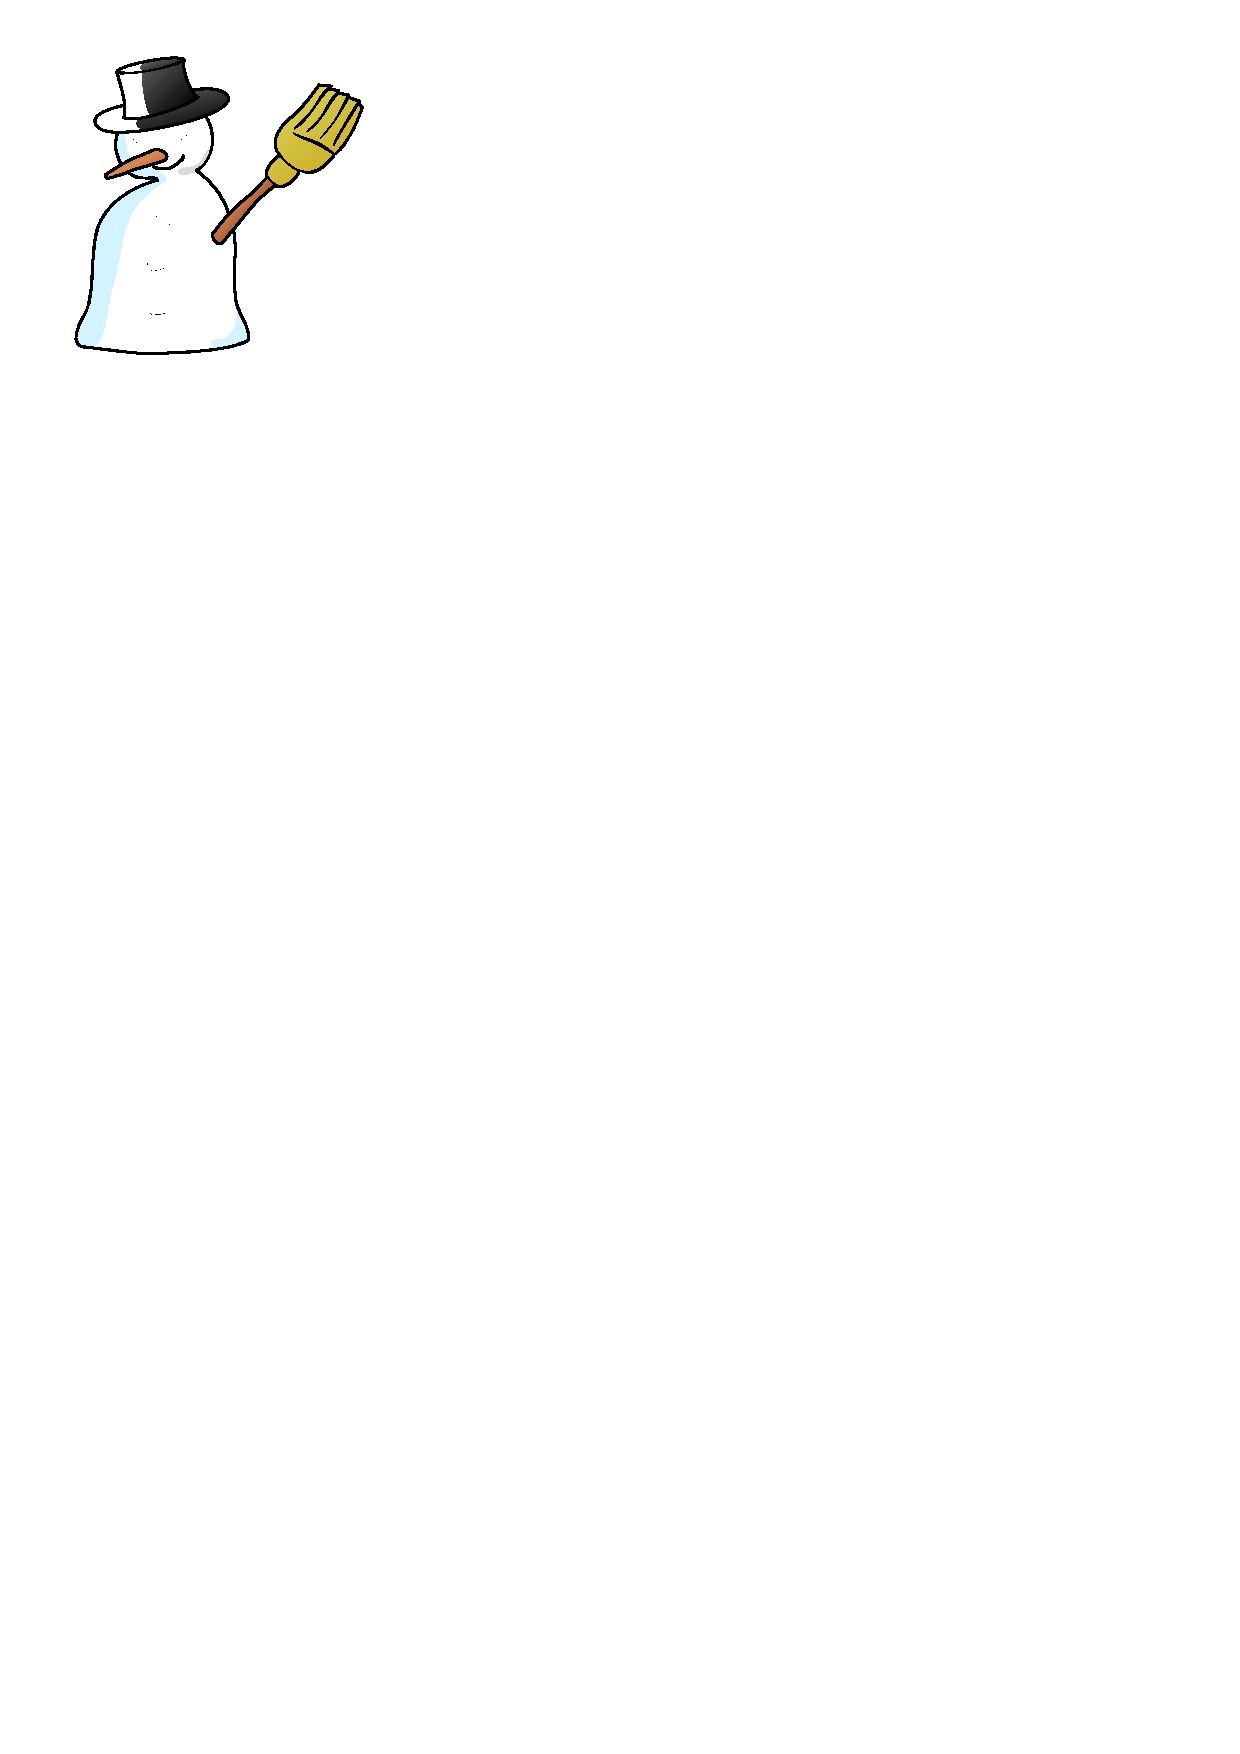
\includegraphics[width=2cm]{snowman-vectorial}
%   \caption{A snow-man}
% \end{wrapfigure}	
% 
% \noindent\verb!\usepackage{wrapfig}!\\
% This then gives you access to:\\
% \verb!\begin{wrapfigure}[lineheight]{alignment}{width}!\\
% Alignment can normally be either ``l'' for left, or ``r'' for right. Lowercase ``l'' or ``r'' forces the figure to start precisely where specified (and may cause it to run over page breaks), while capital ``L'' or ``R'' allows the figure to float. If you defined your document as twosided, the alignment can also be ``i'' for inside or ``o'' for outside, as well as ``I'' or ``O''. The width is obviously the width of the figure. The example above was introduced with:
% \lstset{language=TeX, morekeywords={\begin,\includegraphics,\caption}, caption=Wrapfig Example, label=lst:latex_example}
% \begin{lstlisting}
% 	\begin{wrapfigure}{l}{2.5cm}
% 	  \centering
% 	    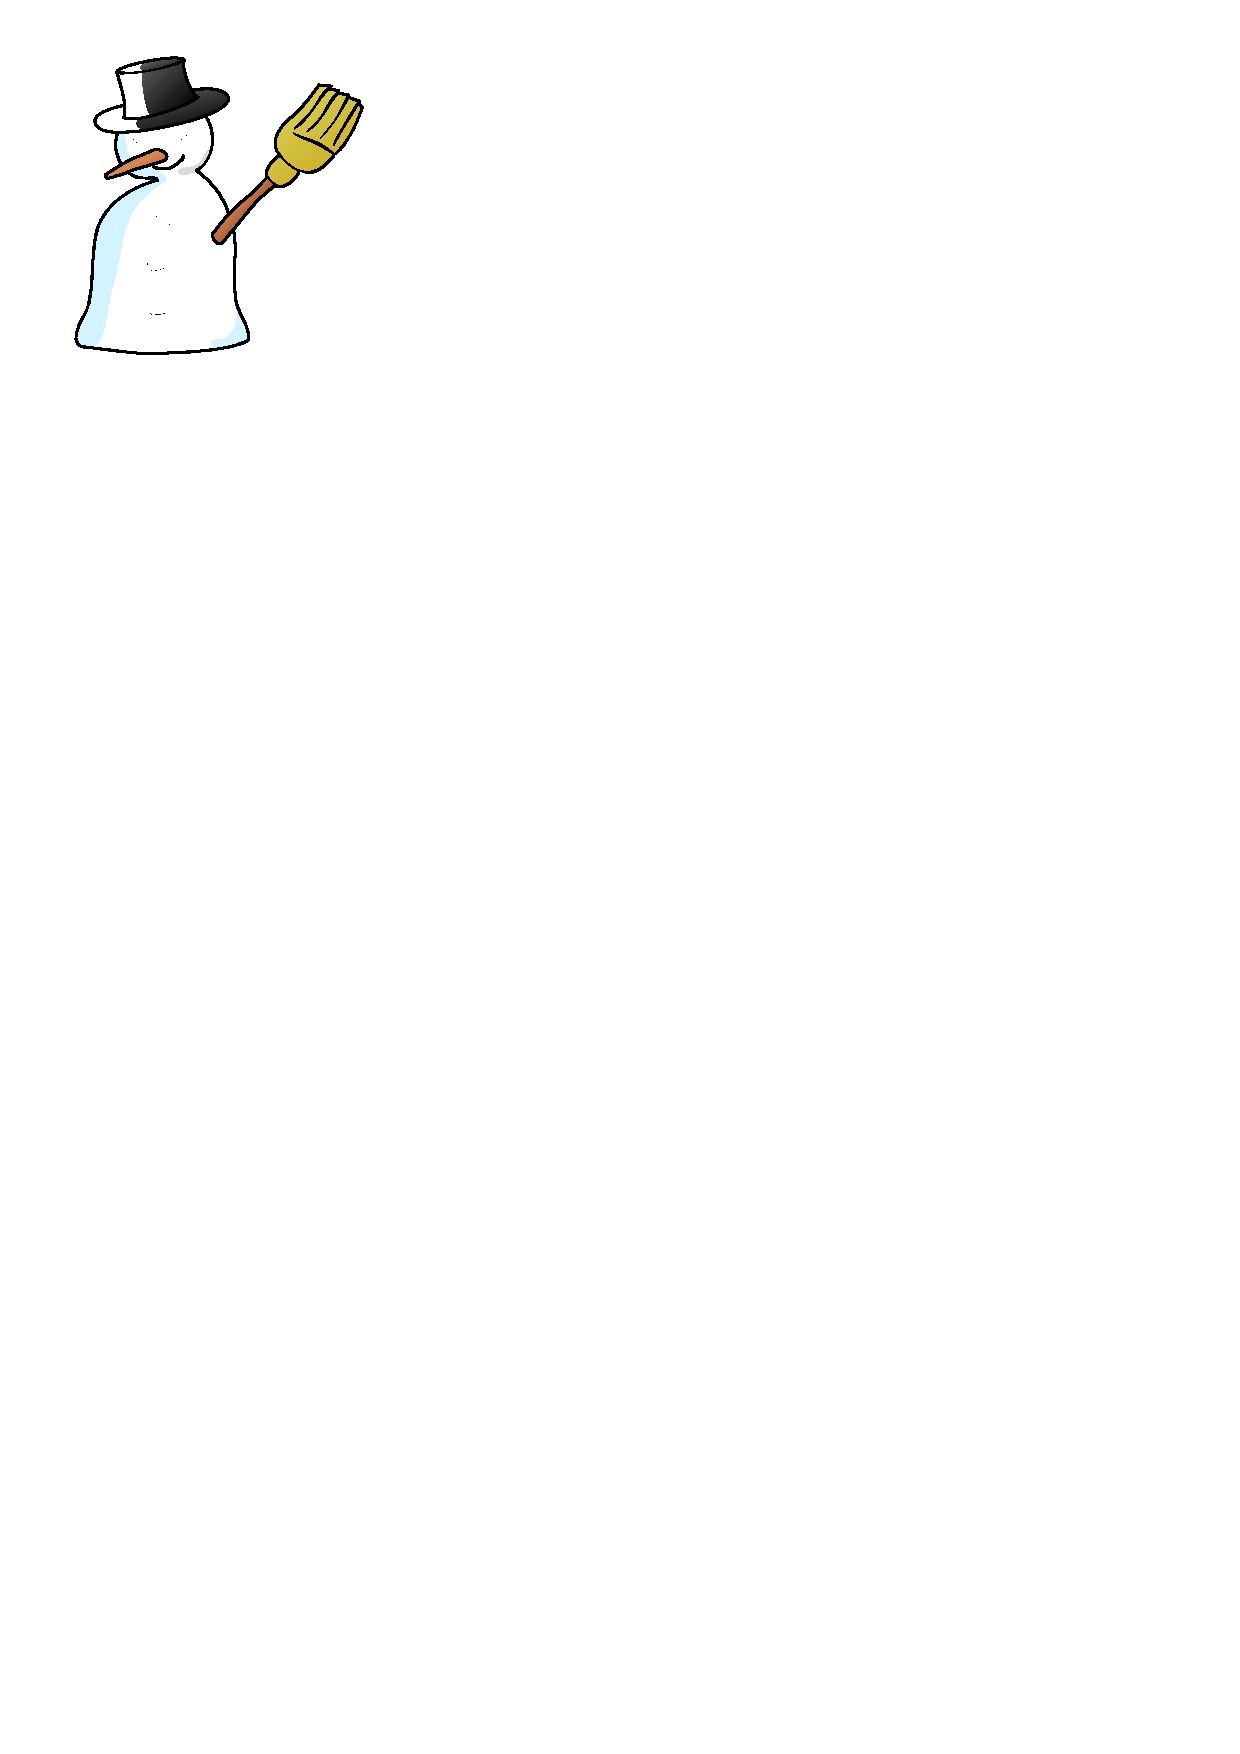
\includegraphics[width=2cm]{snowman-vectorial}
% 	  \caption{A snow-man}
% 	\end{wrapfigure}	
% \end{lstlisting}

% subsection inserting_images_wrapped_with_text (end)

% section floats_figures_and_captions (end)

